% Written by
% Omur Ugur
% Email: ougur@metu.edu.tr
%
% can be any class (with options) hopefully
% a4paper and 12pt options are not mandatory, but preferred 
\documentclass[a4paper, 12pt]{article} % for a simple paper
%\documentclass[a4paper, 12pt]{report} % for a term project

% Language Specific (generally not neede):
%\usepackage[T1]{fontenc} 
%\usepackage[utf8]{inputenc}
% it is important that you load this package: iamPaperStyle.sty
\usepackage{iamPaperStyle} %includes also graphicx.sty and xcolor.sty

% any other styles you need
% not mandatory, but helful 
\usepackage{graphicx} % although loaded by iamPaperStyle.sty
\usepackage{amsmath, amssymb, amsthm} % others
\usepackage{hyperref} % other

% you may use a bit larger area on an a4paper in the document by
\usepackage{a4wide} % not necessary but generally useful
\usepackage{caption}
\usepackage{subcaption}

% now you may begin
\begin{document}

\studentName{Uğurcan Özalp}
\advisorName{Prof.~Dr.~Ömür Uğur}
% Your Department: 
% Scientific Computing, 
% Financial Mathematics, 
% Cryptography, or 
% Actuarial Sciences
\departmentName{Scientific Computing}
% Type of the Document:
% Preprint # may not work as expected (to-do)
% Qualification in PhD
% Report for Thesis Monitoring Committee
% Term Project
% Draft of a Manuscript
\paperType{Draft of a Manuscript}


\paperTitle{%
	Bipedal Robot Walking by Reinforcement Learning in Partially Observed Environment
}

\paperAuthor{%
  U. \"{O}zalp\footnote{%
    Middle East Technical University, Institute of Applied
    Mathematics, 06800 \c{C}ankaya, Ankara, Turkey. \hfill
  \emph{E-Mail}: \texttt{ugurcan.ozalp@metu.edu.tr}},
	% possibly your advisor and co-advisor
  \"{O}. U\u{g}ur\footnote{Middle East Technical University, Institute of Applied
  Mathematics, 06800 \c{C}ankaya, Ankara, Turkey. \hfill
  \emph{E-Mail}: \texttt{ougur@metu.edu.tr}}
}
% abstract should not be large to fit in the title/front page
\paperAbstract{%
Deep Reinforcement Learning methods on mechanical control have been successfully applied in many environments and used instead of traditional optimal and adaptive control methods for some complex problems. 
However, Deep Reinforcement Learning algorithms do still have some challenges. 
One is to control on partially observable environments. 
When an agent is not informed well of the environment, it must recover information from the past observations. 
In this thesis, walking of Bipedal Walker Hardcore (OpenAI GYM) environment, 
which is partially observable, 
is studied by two continuous actor-critic reinforcement learning algorithms; Twin Delayed Deep Determinstic Policy Gradient and Soft Actor Critic.
Several neural architectures are implemented. 
The first one is Residual Feed Forward Neural Network under the observable environment assumption, 
while the second and the third ones are Long Short Term Memory and Transformer using observation history as input to recover the hidden information due to the partially observable environment. 
}

\paperKeywords{%
  deep reinforcement learning, partial observability, robot control, actor-critic methods, long short term memory, transformer
}

\paperDate{July 2021}

 % edit this file or see the lines below
%%%%%%%%%%%%%%%%%%%%%%%%%%%%%%%%%%%%%%%%%%%%%%%%%%%%%%%%%%%%%%%%%%%%%
% you may also use the predefined macros also here to over-write the
% info in the included file newPreprintDetails.tex

% \studentName{Ömür Uğur}
% \advisorName{Prof.~Dr.~Hamdullah Yücel}
% \departmentName{Scientific Computing}
% \paperType{Draft of a Manuscript}
% \paperTitle{This is the Title}
% \paperAuthor{\"{O}. U\u{g}ur, A. Mehmet}
% \paperAbstract{This is the Abstract} 
% \paperKeywords{Keyword 1, no keyword, illegalWord}
% \paperDate{April 2013} 

%%% mandatory:
\makePaperCoverPage
% for printing (and submitting) uncomment below (to have a sigle title page)
%\blankpage
%%%%%%%%%%%%%%%%%%%%%%%%%%%%%%%%%%%%%%%%%%%%%%%%%%%%%%%%%%%%%%%%%%%%%


%%%%%%%%%%%%%%%%%%%%%%%%%%%%%%%%%%%%%%%%%%
% The rest of the manuscript is trivial...
%%%%%%%%%%%%%%%%%%%%%%%%%%%%%%%%%%%%%%%%%%
% Hoever, try not to use commands like
% \title, \author, \date, \maketitle or \tableofcontents
% unless you need them of course: 
% you might need a title and a table of contents
% at the begining sometimes
%\title{Title of the Manuscript}
%\author{Author Name Surname}
%\date{\today}
%\maketitle

% if necessary (suggested in a simple paper submitted to IAM}
\makeTitle % don't use this if this is a term project
\tableofcontents % will be a separate page in case of term project


%%%%%%%%%%%%%%%%%%%%%%%%%%%
% CONTENT OF THE MANUSCRIPT
%%%%%%%%%%%%%%%%%%%%%%%%%%%

% instead of typing here inside this document
% we suggest you to include or input a
% separate document of yours:
% \input{yourdocname}

% For Reports un comment \chapter{}
%\chapter{In case of a Report Chapter is needed}
%		\label{chap:ReportIntro}

\section{Introduction} \label{sec:first_intro}

Humans and animals exhibit several different behaviours in terms of 
interaction with environment, such as utterance and movement. 
Their behavior is based on past experience, the situation they are in  and their objective. 
Like humans and animals, an intelligent agent is expected to take 
action according to its perception based on some objective. 
A major challenge in Machine Learning to create agents that will 
act more natural and humanlike. 
As a subfield of ML, Reinforcement Learning (RL) allows an 
agent to learn how to control (or act) itself in different situations by interacting with the environment. In RL, environment is modeled to give reward (or punishment) to agent 
according to environmental state and agent actions, and agent focuses
on learning to predict what actions will lead to highest reward 
(or lowest punishment, based on its objective) in the future using past experience. 

Traditional RL algorithms need feature engineering from observations. 
For complex problems, the way to extract features is ambiguous or 
observations are not enough to create a good model. 
In contrast to traditional methods, Deep Neural Networks (DNNs) allows to extract 
high level features from data with large state-space 
(pixelwise visual, many kinematic sensors etc.) and missing  observations.
Along with recent developments in DNNs, Deep Reinforcement Learning (DRL)
allows an agent to interact with the environment in a more complex way.

Since its discovery, robots have been crucial devices for the human race, whether smart or not. 
Intelligent humanoid and animaloid robots have been developed since early 1980s. 
This type of robots has legs unlike driving robots. 
Since most of the world terrain is unpaved, this type of robots are good alternative to driving robots. 
Locomotion is a major task for such robots. Stable bipedal (2 legged)  walking 
is one of the most challenging problem among the control problems. 
It is hard to create accurate model due to high order of dynamics,  friction and discontinuities. 
Even further, the design of walking controller using traditional methods is difficult due to the same reasons. 
Therefore, for bipedal walking, DRL approach is an easier choice if a simulation environment is available. 

In this work, Bipedal Locomotion is investigated through \textit{BipedalWalker-Hardcore-v3} \cite{noauthor_bipedalwalkerhardcore-v2_2021} environment of open source GYM library \cite{brockman_openai_2016} by DRL. 
Our contributions are as follows:
\begin{itemize}
	\item Sequential neural networks are used (LSTM and Transformer) for solution, along with Residual Feed Forward Neural Network.
	\item Twin Delayed DDPG (TD3) and Soft Actor-Critic (SAC) algorithms are used and compared.
	\item Reward shaping and small modifications are applied on environment to hinder possible problems.
\end{itemize}

\section{Environment Details}

\subsection{Dynamics}

\textit{BipedalWalker} environments~\cite{noauthor_bipedalwalker-v2_2021, noauthor_bipedalwalkerhardcore-v2_2021} are parts of Gym environment library. 
One of them is classical where the terrain is relatively smooth, while other is a hardcore version containing ladders, stumps and pitfalls in terrain. 
Dynamics of the robot are exactly identical in both environments. 
The robot has kinematic and lidar sensors. 
It is modeled as Markov Decision Process with deterministic dynamics.

Those environments have continuous action and observation space. 
\textbf{Observation Space} contains hull angle, hull angular velocity, hull translational velocities, joint positions, joint angular speeds, leg ground concats and 10 lidar rangefinder measurements.
The robot has 2 legs with 2 joints at knee and hip. Torque provided to knee and pelvis joints of both legs. These 4 torque values forms  \textbf{Action Space}.

For both settings, the task is to move the robot forward as much as possible.
Snapshots for both environments are depicted in Figure \ref{fig:bipedal_walkers}.

\begin{figure}
	\begin{subfigure}{.5\textwidth}
		\centering
		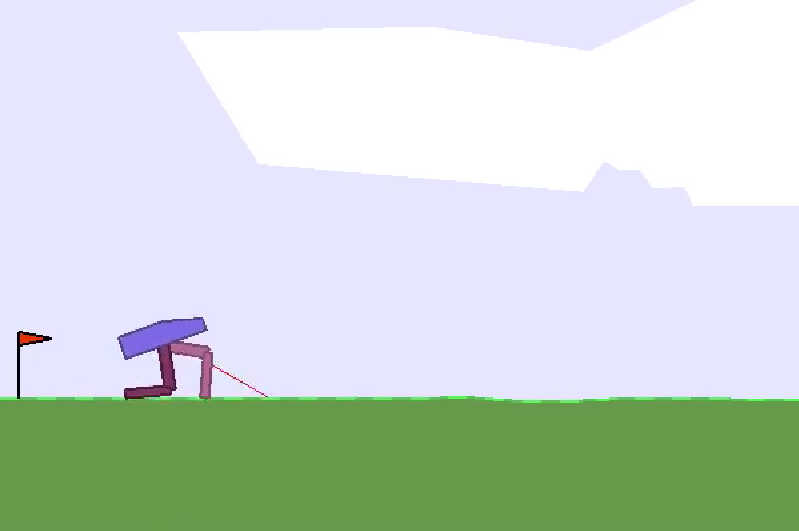
\includegraphics[width=0.9\linewidth]{figures/bipedal/classic.png}
		\caption{BipedalWalker-v3 Snapshot~\cite{noauthor_bipedalwalker-v2_2021}}
		\label{fig:bipedal_walker_classic}
	\end{subfigure}
	\begin{subfigure}{.5\textwidth}
		\centering
		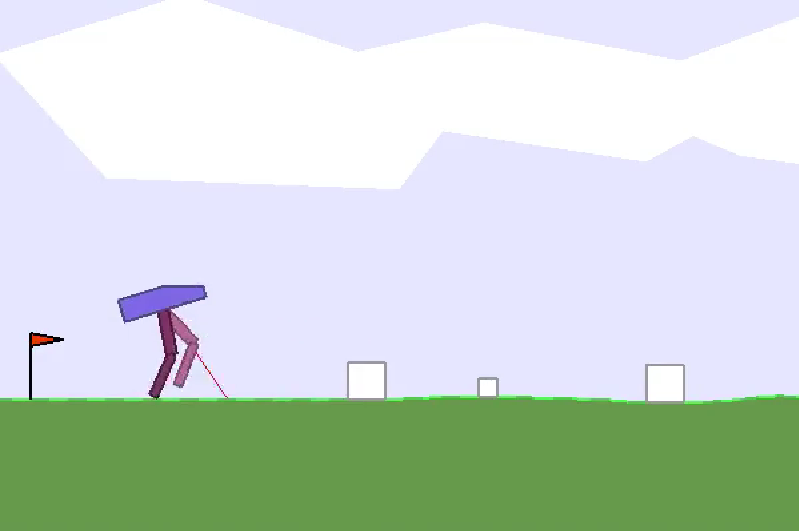
\includegraphics[width=0.9\linewidth]{figures/bipedal/hardcore.png}
		\caption{BipedalWalkerHardcore-v3 Snapshot~\cite{noauthor_bipedalwalkerhardcore-v2_2021}}
		\label{fig:bipedal_walker_hardcore}
	\end{subfigure}
	\caption{Bipedal Walkers Snapshots}
	\label{fig:bipedal_walkers}
\end{figure}

\subsection{Difficulties}

Locomotion of the Bipedal Walker is a difficult control problem due to following reasons: 
\begin{itemize}
	\item \textbf{Nonlinearity}: The dynamics are nonlinear, unstable and multimodal. 
	Dynamical behavior of robot changes for different situations 
	like ground contact, single leg contact and double leg contact.
	\item \textbf{Uncertainity}: The terrain where the robot walks may vary. 
	Designing a controller for all types of terrain is difficult.
	\item \textbf{Reward Sparsity}: Overcoming some obstacles requires a specific maneuver, which is hard to explore sometimes.	
	\item \textbf{Partially Observability}: The robot observes 
	ahead of it with lidar measurements and cannot observe behind. 
	In addition, it lacks of acceleration sensors.
\end{itemize}

These reasons make it hard to implement analytical methods for control tasks. 
However, approach can easily overcome nonlinearity and uncertainity problems.

On the other hand, reward sparsity problem brings local minimums to objective function of optimal control. It can be solved by a good exploration strategy and reward shaping. 

For the partial observability problem, more elegant solution is required. 
This is achieved by creating a belief state from the past observations to inform the agent. 
Agent uses this belief state to choose how to act. 
If belief state is evaluated sufficiently, 
this increases performance of the agent.
However, relying on observations is also possible, 
and this may be enough sometimes if advanced type of control is not required. 

\section{Reinforcement Learning}

\textbf{Reinforcement Learning} is the closest kind of learning demonstrated by humans and animals 
since it is grounded by biological learning systems. 
It is based on maximizing cumulative reward over time to make agent 
learn how to act in an environment~\cite{sutton_reinforcement_1998}. 
Each action of the agent is either rewarded or punished according to a reward function. 
The agent explores environment by taking various actions in different states to gain experience, based on trial-and-error. 
Then it exploits experiences to get highest reward from the environment considering instant and future rewards over time. 

RL is a stochastic control process. 
At time $t$, the agent starts with state $s_t \in \mathcal{S}$ and observes $o_t \in \mathcal{O}$, 
then it takes an action $a_t \in \mathcal{A}$ according to its policy $\pi$ and obtains a reward $r_t \in \mathbb{R}$ at time $t$. 
Then state transition to $s_{t+1} \in \mathcal{S}$ occurs as a consequence of the action and the agent gets the next observation $o_{t+1} \in \mathcal{O}$. 
Along with state transitions, the agent is expected to develop (learn) a policy function 
$\pi \colon \mathcal{S} \rightarrow \mathcal{A}$ which maps 
inputs (observations) $s \in \mathcal{S}$ to outputs (actions) $a \in \mathcal{A}$.

\subsection{Policy Learning}

Policy learning is achieved by maximization of the value function $V^{\pi}(s)$ (cumulative reward) for all possible states, which depends on policy $\pi$. 

\section{Twin Delayed Deep Deterministic Policy Graidient}

\section{Soft Actor-Critic}

\section{Neural Networks}

\subsection{Residual Feed Forward Neural Network}

\subsection{Long Short Term Memory}

\subsection{Transformer}

\section{Proposed Method}

\section{Conclusion}

\section{References}

%%%%%%%%%%%%%%%%%%%%%%%%%%%%
% CONTENT ENDS HERE (almost)
%%%%%%%%%%%%%%%%%%%%%%%%%%%%



%%% The following way of Bibliography is not recommended
%\begin{thebibliography}{99}
	%\bibitem{bertcs96}  G. Berkooz,  P. Holmes and  J.L.  Lumley.
  %Turbulence, Coherent Structuress, Dynamical Systems and Symmetry,
  %Cambridge University Press: Cambridge Monographs on Mechanics,
  %1996. 
%
	%\bibitem{fukisr90}  K. Fukunaga. Introduction to statistical pattern
  %recognition. Computer Science and Scientific Computing. 
	%Academic Press Inc., Boston, MA, second edition, 1990.
%\end{thebibliography}

%
% References in Bibtex format goes into below 
% indicated file with .bib extension
\bibliography{myBiblio} % filename: myBiblio.bib
% You can use full name of authors, 
% however most likely some of the Bibtex entries you will find, 
% will use abbreviated first names.
% If you don't want to correct each of them by hand, 
% you can use abbreviated style for all of the references
% \bibliographystyle{abbrv}
% However, IAM suggests to use
\bibliographystyle{iamBiblioStyle} % better than to use {plain or abbrv}

%%% APPENDIXES in case you need
%\appendix
%
% input your appendix
% If you are not using minted style, then comment the first appendix below
% otherwise uncomment.
%uncomment%  \chapter{Proof of Some Theorem}
\label{app:mintedCodes}

This is appendix text.

\definecolor{myBgColour}{rgb}{0.99,0.99,0.99} % almost white

\setminted[python]{frame=single,
framesep=2mm,
baselinestretch=1.1,
bgcolor=myBgColour,
fontsize=\footnotesize,
linenos, autogobble,
python3=true}

\setminted[matlab]{frame=single,
framesep=2mm,
baselinestretch=1.1,
bgcolor=myBgColour,
fontsize=\footnotesize,
linenos, autogobble,
python3=true}

%\captionsetup[Listing]{format=plain,font={small},labelfont={bf}, aboveskip=-5px}
%\renewcommand{\theListing}{{\arabic{Listing}}}
%\setcounter{Listing}{0}


However, we place a python code here with a listing environment
Listing~\ref{lst:first}.	

\begin{listing}	
\begin{minted}{python}
# Python program to check if the input number is prime or not

num = 407

# take input from the user
# num = int(input("Enter a number: "))

# prime numbers are greater than 1
if num > 1:
   # check for factors
   for i in range(2,num):
       if (num % i) == 0:
           print(num,"is not a prime number")
           print(i,"times",num//i,"is",num)
           break
   else:
       print(num,"is a prime number")
       
# if input number is less than
# or equal to 1, it is not prime
else:
   print(num,"is not a prime number")
\end{minted}
\caption{This is the caption of this Listing environment\label{lst:first}}
\end{listing}

Also we wish to insert a MATLAB code, too.

\definecolor{myBackgroundColour}{rgb}{0.9,0.9,0.9} % almost gray
\begin{minted}[
frame=lines,
framesep=2mm,
baselinestretch=1.2,
bgcolor=myBackgroundColour,
fontsize=\footnotesize,
linenos
]{matlab}
function result = myprime(n)
% MATLAB program to check if the input number is prime or not

%% initially set output flag to true
 result = true;
%% iterate over all positive integers 2,3,...,n-1
%% if n is not divisible by any of these factors....it is prime
 if (n == 1)
     result = 'false';
 elseif (n == 2)
     result = 'true';
 else 
    for i=2:n-1,
        if (mod(n,i)==0)
           result = 'false';
        end
    end
 end
%% return "true" or "false" instead of 1 or 0  
 if (result)
    result = 'true';
 else
    result = 'false';
 end
\end{minted}


Furthermore, here are two files (myPythonCode.py and myMatlabCode.m) included.

\inputminted[
frame=single,
framesep=2mm,
baselinestretch=1.2,
bgcolor=myBackgroundColour,
fontsize=\footnotesize,
linenos
]{python}{myPythonCode.py}

\definecolor{myRed}{rgb}{0.95,0.1,0.1}

\begin{listing}
\inputminted[frame=single, linenos, bgcolor=myRed]{matlab}{myMatlabCode.m}
\caption{Here is the caption again}
\end{listing} % includes minted package examples!
%\chapter{Proof of Some Theorem}
\label{app:somethms}

This is appendix text.

\begin{listing}
  %\VerbListingBoxed{myMatlabCode.m}
  \VerbatimInput{myMatlabCode.m}
	%\inputminted{matlab}{myMatlabCode.m} % only if minted is used!
  %\VerbListing{myMatlabCode.m}
\caption{The \texttt{lintest} function in a floating ``listing'' environment.}
\label{mfile:linetest-3}
\end{listing}




\end{document}

